\documentclass{article}
\usepackage{amsthm}
\usepackage{amsmath}
\usepackage{amssymb}
\usepackage{graphicx}
\usepackage{algorithm}
\usepackage{algorithmic}
\usepackage{url}
\usepackage{tikz}
\newtheorem{mydef}{Definition}
\newtheorem{prop}{Property}
\newtheorem{theorem}{Theorem}
\newtheorem{proposition}{Proposition}
\newtheorem{problem_statement}{Problem Statement}
\title{Incremental Algorithm for Architecture Selection of Convolutional Neural Networks}
\begin{document}

\maketitle

We will start with some discussion of gradient-boosting algorithm which will lead us nicely to convex neural networks. We will then discuss difference of convex programming in order to solve the optimization problem in convex neural network efficiently. Finally, we will extend the algorithm of convex neural networks to convolutional neural networks (CNNs) having filters and multiple layers.

\section{Gradient-boosting algorithm}
\label{sec:grad_boosting}
We assume our function approximator to be of the form:

\begin{equation}
	F({\bf x}) = f_0({\bf x}) + \beta_1 h_1({\bf x, a_1}) + \beta_2 h_2({\bf x, a_2}) + \dots + \beta_M h_M({\bf x, a_m})  
\end{equation}

where $f_0({\bf x})$ is the initial guess and $\beta_i h_i({\bf x, a_i})$ are successive boosts/increments. The principle idea behind gradient-boosting algorithm is to learn the base-learners greedily, at each step selecting the base-learner which correlates best with the negative gradient of the errors. This is like gradient-descent - instead of adding parameter update in the classical case, here we are adding function update (under the constraint that the base-learner is of certain parametric form).

\begin{algorithm}
\caption{{\bf GradientBoosting} \cite{friedman2001greedy}}\label{algo:gradient_boosting}
\begin{algorithmic}[1]
\STATE {\bf Input:} A loss function $Q$, the form of base learners $h_{i}({\bf x, a})$, number of iterations $M$
\STATE Set $F_0({\bf x}) = argmin_{\beta}  \sum_{j = 1}^{N} Q(y_j, \beta)$
\FOR{$m = 1, 2 .., M$}
\STATE Calculate $-{\bf g}_m({\bf x}) = - \frac{\partial Q(y, F{\bf(x)}}{\partial F{\bf(x)}}|_{F({\bf x}) = F_m({\bf x})}$
\STATE ${\bf a}_m$ = $argmin_{{\bf a}, \beta} \sum_{j = 1}^{N} (- g_m({\bf x_j}) - \beta h_m({\bf x_j;a}))^2$
\STATE $\beta_m = argmin_{\beta}  \sum_{j = 1}^{N} (- g_m({\bf x_j}) - \beta h_m({\bf x_j;a_m}))^2$
\STATE Set $F_m({\bf x}) = F_{m - 1}({\bf x}) + \beta_m h_m({\bf x, a_m})$
\ENDFOR
\STATE Return $F({\bf x}) = f_0({\bf x}) + \sum_{j = 1}^{M} \beta_j h_j({\bf x, a_j})$
\end{algorithmic}
\end{algorithm}

Note that after the selection of $h_m({\bf x; a})$, when only $\beta_m$ is optimized (as in above), the algorithm is called greedy ``stagewise" approach. A less greedy approach is to optimize $\beta_1, \dots, \beta_m$ at the $m$-th iteration. This less greedy approach is called a ``stepwise" approach.   

\section{Convex Neural Networks}

We are now in a position to discuss the algorithm (referred to as ConvexNN here) stated in \cite{bengio2005convex}. ConvexCNN uses the gradient-boosting approach to build a one hidden-layer NN in a greedy ``stepwise" manner. In this case, a neuron corresponds to the base learner $h_m({\bf x; a})$ in section~\ref{sec:grad_boosting}. Given a dataset, a loss function and a regularization factor, the algorithm returns a network with an optimum number of nodes in the hidden layer and the set of weights (input to hidden layer, hidden layer to output).

\begin{algorithm}
\caption{{\bf ConvexNN}}\label{algo:ConvexNN}
\begin{algorithmic}[1]
\STATE {\bf Input:} Training dataset $D = \{({\bf x_1}, y_1), \dots, ({\bf x_n}, y_n)\}$, convex loss function $Q$, and scalar regularization penalty $\lambda$. $s$ is some non-linear activation function 
\STATE Select ${\bf v_1}$ to some initial value and select $w_1 = argmin_{w1} \sum_t Q(w_1.s({\bf v}_1 \cdot {\bf x}_t), y_t) + \lambda |w_1|^2$
\FOR{$i = 2,3 .., $}
\STATE Let $q_t = \frac{\partial Q(y, y_t)}{\partial y}|_{\bf x = x_t}$ where $y = \sum_{j = 1}^{i - 1} w_j . s({\bf v_j} \cdot \bf{x})$
\STATE Select best ${\bf v_i}$ by maximizing $\sum_{t} q_t s({\bf v}_i \cdot {\bf x}_t) - \lambda ||{\bf v_i}||^2$ 
\STATE If $\sum_{t} q_t s(v_i \cdot {\bf x}_t) - \lambda ||{\bf v_i}||^2 < \lambda$, {\bf stop}
\STATE Select $w_1, ...., w_i$ by minimizing $C =  \sum_t Q(\sum_{j = 1}^{i} w_j \cdot s({\bf v}_j \cdot {\bf x}_t), y_t) + \lambda \sum_{j = 1}^{i}|w_j|^2$
\ENDFOR
\STATE Return the predictor $y({\bf x}) = \sum_{j = 1}^{i} w_j \cdot h_j({\bf x})$ 
\end{algorithmic}
\end{algorithm}

Note that (7) in algorithm~\ref{algo:ConvexNN} is convex optimization in $w_1, \dots, w_i$. This is because the first term $Q$ is taken to be convex in $y$, which is linear combination of weights (convex composition of affine transform preserves convexity). The second term is also convex in weights (each term has double derivative $>$ 0 since $\lambda$ is taken to be positive).

It is instructive to note that (5) tries to select the ${\bf v}_i$ which maximises the (expected) correlation between $q$ and $s({\bf v}_i, {\bf x})$. Let $\mu(X)$ represent the mean of r.v $X$ and $\sigma(X)$ represent its standard deviation. Correlation is defined as:

\begin{align}
corr(X, Y) &= \frac{cov(X, Y)}{\sigma(X)\sigma(Y)} \\
	&= \frac{E[(X - \mu(X))(Y - \mu(Y))]}{\sigma(X)\sigma(Y)} \\
	&= \frac{E[XY] - \mu(X)\mu(Y)}{\sigma(X)\sigma(Y)} 
\end{align}  

Using above:

\begin{align}
\label{eq:correlation}
corr(q, s({\bf v}_i, {\bf x})) &= \frac{E[q \cdot s({\bf v}_i, {\bf x})] - \mu(q)\mu(s({\bf v}_i, {\bf x}))}{\sigma(q)\sigma(s({\bf v}_i, {\bf x}))} 
\end{align}  

In step (5) of algorithm \ref{algo:ConvexNN}, the objective function represents the above correlation (approximately). The first term corresponds to $E[q \cdot s({\bf v}_i, {\bf x})]$ and the second term is a proxy for $\mu(s({\bf v}_i, {\bf x}))$. Note that if $s()$ is tanh or sign activation, the output is between 1 and -1, so the regularizer term is not required. Another way to think is that there are many  ${\bf v}_i$ which can make $\mu(s({\bf v}_i, {\bf x}))$ parallel to $q$ and we want ${\bf v}_i$ of small magnitude. Also observe that this objective of correlation maximization is different from the least squares based criterion in step (5) of algorithm \ref{algo:gradient_boosting}. It needs to be seen which optimization is easier in practice.

\section{Difference of Convex Programming}
\label{sec:DC_programming}

Some non-convex functions can be decomposed into difference of convex functions (what is the characterization of this class?). To solve the minimization problem for such non-convex functions, we can linearize the concave part at a particular point, minimize the resulting convex overestimate (convex + linear), move to the minima and linearize the concave function at this point again. The algorithm continues iteratively until the improvement is very small.

\begin{algorithm}
\caption{{\bf Difference of Convex Programming}}\label{algo:dc_programming}
\begin{algorithmic}[1]
\STATE {\bf Input:} $f({\bf x})$, number of iterations $N$, stopping threshold $\lambda$
\STATE Decompose $f({\bf x}) = g({\bf x}) + h({\bf x})$ where $g({\bf x})$ is convex and $h({\bf x})$ is concave
\STATE Select a starting point $\bf x_0$ 
\FOR{$i = 1, 2 .. $}
\STATE Linearize $h({\bf x})$ by $h_i({\bf x})= h({\bf x}_i) + \nabla h({\bf x})|_{\bf x = x_i}^T ({\bf x} - {\bf x_i})$
\STATE Set ${\bf x}_i = argmin_{{\bf x}} g({\bf x}) + h_i({\bf x})$ by solving the convex optimization problem
\STATE If $f({\bf x_{i - 1}}) - f({\bf x_i}) < \lambda$, {\bf stop}
\ENDFOR
\end{algorithmic}
\end{algorithm}

Consider the objective function in (6) of algorithm \ref{algo:dc_programming}:

\begin{equation}
f_i({\bf x}) = g({\bf x}) + h_i({\bf x})
\end{equation}

$f_i({\bf x})$ is a convex function (sum of convex and linear functions). Moreover $f_i({\bf x})$ is a global overestimate of $f({\bf x})$, because $h_i({\bf x})$, being tangent at ${\bf x}_i$, is an overestimate of $h({\bf x})$ globally. If $f_i({\bf x})$ is of the following form, then it can be minimized using efficient algorithms like block-coordinate frank-wolfe (BCFW):

\begin{equation}
min_{\bf w} \frac{1}{N} \sum_{i = 1}^{N} max_j ({\bf a}_{ij}^T{\bf w} + b_{ij}) + \frac{\lambda}{2} ||{\bf w}||^2
\end{equation}

The above is a convex function. Pointwise maximum of linear functions is convex. Positive weighted sum of convex functions is convex. Hence, first term is convex. Second term is convex since $||W||^2$ can be thought of as $u^T \cdot W \cdot v$ (where $u$ and $v$ are vectors of 1s of appropriate dim) and $\lambda > 0$.

Consider the objective function of (5) of algorithm \ref{algo:ConvexNN}:

\begin{equation}
max_{{\bf v}} \sum_{t} q_t \cdot s({\bf v}.{\bf x}_t) - \lambda ||{\bf v}||^2
\end{equation}

Let us rewrite the above as:

\begin{equation}
min_{{\bf v}} \sum_{t} q'_t \cdot s({\bf v}.{\bf x}_t) + \lambda ||{\bf v}||^2
\end{equation}

where $q'_t = -q_t$. Let

\begin{equation}
Q = \sum_t (\hat{y}_t - y_t)^2 + \lambda ||W||^2
\end{equation}

where $\hat{y}_t$ is the true response for the $t$-th example and $y_t$ is the predicted response. We have:

\begin{equation}
q_t' =  - \frac{\partial Q}{\partial y}|_{y = y_t} = \sum_t 2 \cdot (\hat{y}_t - y_t)
\end{equation}

Let us restrict the activation function to be $s(x) = max(0, x)$ because of its convex piecewise linear nature. The objective function becomes:

\begin{align}
f({\bf v}) &= \sum_{t} q'_t \cdot max(0, {\bf v}.{\bf x}_t) + \lambda ||{\bf v}||^2 \\
&= \sum_{t: q'_t > 0} q'_t \cdot max(0, {\bf v}.{\bf x}_t) + \lambda ||{\bf v}||^2 +  \sum_{t: q'_t \leq 0} q'_t \cdot max(0, {\bf v}.{\bf x}_t) \\
&= g({\bf v}) + h({\bf v})
\end{align}

where $g({\bf v}) = \sum_{t: q'_t > 0} q'_t \cdot max(0, {\bf v}.{\bf x}_t) + \lambda ||{\bf v}||^2 $ is convex and $h({\bf v}) = \sum_{t: q'_t \leq 0} q'_t \cdot max(0, {\bf v}.{\bf x}_t)$ is concave. As an aside, note that checking sign of $q'_t$ is easy - just check if $\hat{y}_t > y_t$. Let us linearize $h({\bf v})$ at a given point ${\bf v}_i$:

\begin{align}
h_i({\bf v})= h({\bf v}_i) + \nabla h({\bf v})|_{\bf v = v_i}^T ({\bf v} - {\bf v_i})
\end{align}

where

\begin{align}
\nabla h({\bf v}) &= \frac{\partial h}{\partial {\bf (v\cdot x)}} \cdot \frac{\partial{\bf (v\cdot x)}}{\partial {\bf v}} \\
\end{align}

\begin{align}
\frac{\partial h}{\partial {\bf (v\cdot x)}} = 
\begin{cases}
0 & if {\bf v\cdot x} < 0 \\
1 & if {\bf v\cdot x} > 0 \\
\end{cases} 
\end{align}

Hence, 

\begin{align}
\nabla h({\bf v})|_{\bf v = v_i} =
\begin{cases}
0 & if {\bf v_i \cdot x} < 0 \\
{\bf x} & if {\bf v_i \cdot x} > 0 \\
\end{cases} 
\end{align}

Given the dataset, we can compute the expectation of $\nabla h({\bf v})|_{\bf v = v_i}$ over ${\bf x}$, i.e, $E_{{\bf x}_t, q'_t < 0}(\nabla h({\bf v})|_{\bf v = v_i})$. The convex function to be minimised now becomes:

\begin{align}
f_i({\bf v}) = \sum_{t: q'_t > 0} q'_t \cdot max(0, {\bf v}.{\bf x}_t) + \lambda ||{\bf v}||^2 + h({\bf v}_i) + \nabla h({\bf v})|_{\bf v = v_i}^T ({\bf v} - {\bf v_i})
\end{align}

Removing the constant terms:

\begin{align}
f'_i({\bf v}) = \sum_{t: q'_t > 0} q'_t \cdot max(0, {\bf v}.{\bf x}_t) + \lambda ||{\bf v}||^2 + (\nabla h({\bf v})|_{\bf v = v_i}^T) {\bf v}
\end{align}

The above objective function is composed of quadratic and linear terms in ${\bf v}$ and there exists quadratic convex programming algorithms to minimise it efficiently.

\section{Greedy Algorithm for CNN Architecture}

In this section, we extend ConvexNN to CNNs. Instead of adding one neuron at a time, we add one filter greedily in this case. Importantly, at each step we decide whether to add a filter to the current layer or whether to start a new layer and add the filter there. The CNN architecture we consider is as follows:

Input -\textgreater [Convolution -\textgreater ReLU] -\textgreater ..... -\textgreater [Convolution - \textgreater ReLU] -\textgreater Output

We make an assumption:

\begin{enumerate}
\item Filter size, max pool size and the stride are the same at each layer. Also, these are available via an oracle \texttt{FindBestFilterPoolSize}
\end{enumerate}

Some comments on notation. We use ${\bf X}_t$, instead of ${\bf x}_t$ to denote the input in this case, to emphasize that inputs to CNNs are best thought of as matrices, rather than vectors. ${\bf V}_{i, j}$ denotes the weight matrix corresponding to the $j$-th filter in the $i$-th layer. $\texttt{nLayer}$ stands for  number of layers and $\texttt{nFilter}$ for number of filters in $\texttt{nLayer} - 1$-th layer at the current point in network evolution. ${\bf U}$ denotes output of layer $\texttt{nLayer} - 2$ (input to $\texttt{nLayer} - 1$) and ${\bf Z}$ denotes the output of layer $\texttt{nLayer} - 1$.

\iffalse
Given a dataset, cost function and regularization term, we want to learn the number of convolutional layers, number of filters in each layer, filter size and pooling size of each filter, and the weights corresponding to each filter and the output layer. The basic structure of our network is:

Input -\textgreater [Convolution -\textgreater ReLU -\textgreater Max Pooling] -\textgreater ..... -\textgreater [Convolution - \textgreater ReLU -\textgreater Max Pooling] -\textgreater Output

First of all, let us assume that we have only one convolutional layers and consider the problem of adding filters incrementally to this layer. Also assume that we have a subroutine FindBestFilterPoolSize($i$) which takes as input the index $i$ of a filter in this layer and returns the optimum filter size $f_i$ and max-pool size $p_i$ for the $i$-th filter.

Let $X \in R^{n \times n}$ be the input matrix (assume square) and $y \in R$ be a scalar output. Let $V_i \in R^{f \times f}$ be the shared matrix for the $i$-th filter in the first layer having a filter size of $f$. The output of the filter is a matrix $Z_i = V_i * X \in R^{n \times n}$. ReLU here corresponds to the function $y = max(0, x)$ where $y, x \in R$. Let us denote element-wise ReLU operation on a matrix $A$ by $s(A)$. If the pool size is $p$, we assume the stride is $p$ (non-overlapping). The output of max-pooling for input $Z_i \in R^{n \times n}$ is denoted by $POOL(Z_i) \in R^{n/p \times n/p}$. The output matrix for pooling corresponding to $i$-th filter is denoted by $W_i$.
\fi

\vspace{5mm}
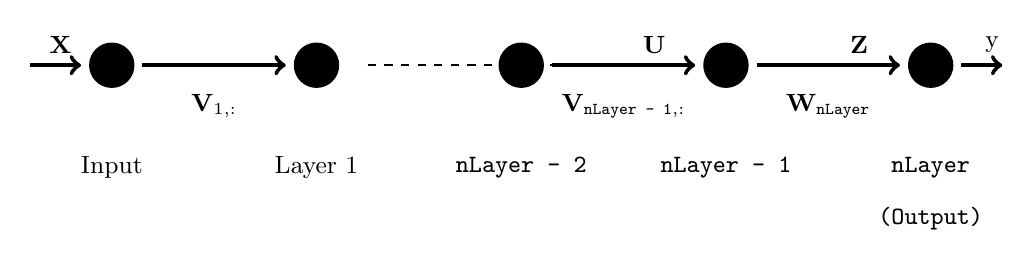
\begin{tikzpicture}[scale=1.3]
\small
%\draw[help lines] (0, 0) grid (10, 2);
\draw [ultra thick] [->] (0.2, 1) -- (0.7, 1);
\node at (0.5, 1.2) {{\bf X}};
\draw [black, fill=black, ultra thick] (1, 1) circle [radius=0.2];
\node at (1, 0) {Input};
\draw [ultra thick] [->] (1.3, 1) --(2.7,1);
\node at (2, 0.6) {${\bf V}_{1, :}$};
\draw [black, fill=black, ultra thick] (3, 1) circle [radius=0.2];
\node at (3, 0) {Layer 1};
\draw [dashed] [thick] (3.5, 1) --(5.5,1);
\draw [black, fill=black, ultra thick] (5, 1) circle [radius=0.2];
\node at (5, 0) {\texttt{nLayer - 2}};
\node at (6.3, 1.2) {{\bf U}};
\draw [ultra thick] [->] (5.3, 1) --(6.7,1);
\node at (6, 0.6) {${\bf V}_{\texttt{nLayer - 1}, :}$};
\draw [black, fill=black, ultra thick] (7, 1) circle [radius=0.2];
\node at (7, 0) {\texttt{nLayer - 1}};
\node at (8.3, 1.2) {{\bf Z}};
\draw [ultra thick] [->] (7.3, 1) --(8.7,1);
\node at (8, 0.6) {${\bf W}_{\texttt{nLayer}}$};
\draw [black, fill=black, ultra thick] (9, 1) circle [radius=0.2];
\node at (9, 0) {\texttt{nLayer}};
\node at (9, -0.5) {\texttt{(Output)}};
\node at (9.6, 1.2) {y};
\draw [ultra thick] [->] (9.3, 1) --(9.7,1);
\end{tikzpicture}

\begin{algorithm}
\caption{{\bf IncrementalCNN}}\label{algo:GreedyCNN}
\begin{algorithmic}[1]
\STATE {\bf Input:} Training dataset $D = \{({\bf X}_1, \hat{y}_1), \dots, ({\bf X}_n, \hat{y}_n)\}$, convex loss function $Q$, and scalar regularization penalty $\lambda$. $s$ is ReLU
\STATE Set \texttt{nLayer} = 1, \texttt{nFilter} = 1
\STATE Select ${\bf V_{1,1}}$ to some initial value and select $W_1 = argmin_{W1} \sum_t Q(y_t, \hat{y}_t) + \lambda ||W_1||^2$ where $y_t$ is predicted output
\WHILE{TRUE}
\STATE Let $q'_t = - \frac{\partial Q(\hat{y}, y)}{\partial y}|_{\bf X = X_t}$. Let ${\bf U_t}$ be the input to and ${\bf Z_t}$ be the output of \texttt{nLayer} - 1
\IF{min $\sum_{t} q'_t s({\bf V} * {\bf U}_t) + \lambda ||{\bf V}||^2$ $<$ min $\sum_{t} q'_t s({\bf V} * {\bf Z}_t) + \lambda ||{\bf V}||^2$}
	\STATE \texttt{nFilter} += 1
	\STATE Get ${\bf V_{\texttt{nLayer - 1}, \texttt{nFilter}}}$
	\STATE If min $\sum_{t} q'_t s({\bf V} * {\bf U}_t) + \lambda ||{\bf V}||^2 < \lambda$, {\bf stop}
\ELSE
	\STATE \texttt{nLayer} += 1, \texttt{nFilter} = 1 
	\STATE Get ${\bf V_{\texttt{nLayer - 1}, \texttt{nFilter}}}$
	\STATE If min $\sum_{t} q'_t s({\bf V} * {\bf Z}_t) + \lambda ||{\bf V}||^2 < \lambda$, {\bf stop}
\ENDIF
\STATE Select ${\bf W}_{\texttt{nLayer}}$ by minimizing $C =  \sum_t Q(\hat{y}_t, y_t) + \lambda ||W||^2$
\ENDWHILE
\STATE Return ${\bf W}_{\texttt{nLayer}}$ and ${\bf V}_{\texttt{1:nLayer-1, :}}$
\end{algorithmic}
\end{algorithm}

\iffalse
\begin{algorithm}
\caption{{\bf IncrementalCNN}}\label{incremental_algo}
\begin{algorithmic}
\STATE {\bf Input:} Training dataset $D = \{(X_1, y_1), \dots, (X_n, y_n)\}$, convex loss function $Q$, and scalar regularization penalty $\lambda$. $s$ is ReLU
\STATE $f_1, p_1$ = FindBestFilterPoolSize(1)
\STATE Select $V_1$ to some initial value and select $W_1 = argmin_{W1} \sum_t Q(W_1.POOL(s(V_1 * X)), y_t) + \lambda |W_1|$
\FOR{$i = 2,3 .., $}
\STATE Let $q_t = Q'(\sum_{j = 1}^{i - 1} W_j . POOL(s(V_j * X), y_t)$ 
\STATE $f_i, p_i$ = FindBestFilterPoolSize($i$)
\STATE Select best $V_i$ by maximizing $\sum_{t} q_t POOL(s(V_i * X))$ using BCFW
\STATE If $\sum_{t} q_t POOL(s(V_i * X)) < \lambda$, {\bf stop}
\STATE Select $W_1, ...., W_i$ by minimizing $C =  \sum_t Q(\sum_{j = 1}^{i} W_j . POOL(s(V_j * X)), y_t) + \lambda \sum_{j = 1}^{i}|W_j|$
\ENDFOR
\end{algorithmic}
\end{algorithm}
\fi

In step (6) algorithm \ref{algo:GreedyCNN}, we solve two minimization problems (using the method outlined in section \ref{sec:DC_programming}) and decide whether to add a filter to current layer or to the next (new) layer by selecting the one which best aligns with $q'_t$. A new layer can be thought of as function transformation. Specifically, let $F_m({\bf x})$ be function approximator in the $m$-th iteration (represented by NN). Let us assume we have one hidden layer and three units in this layer.

\begin{equation}
F_m({\bf x}) = f_1({\bf x})+ f_2({\bf x})  + f_3({\bf x})
\end{equation}

If we add one more filter to this layer:

\begin{equation}
F_{m+1}({\bf x}) = f_1({\bf x})+ f_2({\bf x})  + f_3({\bf x}) + f_4({\bf x})
\end{equation}

To get the best $f_4({\bf x})$, we apply the technique of gradient-boosting in section \ref{sec:grad_boosting} in a straightforward manner. However, if were instead considering adding a new filter/unit in the next layer, $F_{m+1}({\bf x})$ will become a non-linear composition of functions:

\begin{equation}
F_{m+1}({\bf x}) = g_1(f_1({\bf x})+ f_2({\bf x})  + f_3({\bf x}))
\end{equation}

We can rewrite it as

\begin{align}
F_{m+1}({\bf x}) &= g_1({\bf z}) \\
\textrm{where } {\bf z} &= f_1({\bf x})+ f_2({\bf x})  + f_3({\bf x})
\end{align}

Adding a second filter in the new layer leads to:

\begin{align}
F_{m+2}({\bf x}) &= g_1({\bf z}) + g_2({\bf z})\\
\textrm{where } {\bf z} &= f_1({\bf x})+ f_2({\bf x})  + f_3({\bf x})
\end{align}

As we can see from above, given $f_1({\bf x})+ f_2({\bf x})  + f_3({\bf x})$ as fixed, we can now think of our dataset as $\{{\bf z}_t, y_t)\}_{t = 1}^{N}$ (instead of the usual $\{{\bf x}_t, y_t)\}_{t = 1}^{N}$) and apply the gradient boosting technique. The algorithm needs to be extended to max-pooling after ReLU activation.

\section{Experiments}
\label{sec:Experiments}

There are three experiments which can be tried out. The first two are for sanity check and use MLPs, instead of CNNs.

\begin{enumerate}
\item Assume a hihgly non-convex function. Generate training data using it (with added noise). Use our algorithm to build an MLP - observe how wide and deep it builds. Check if predictions match.  
\item Assume a MLP with three layers and a small number of nodes in each layer. Assume random weights. Generate training data from it. Use algorithm to build an MLP. See how it differs from the original MLP.
\item Work with a subset of the MNIST data (say 50 images per class 0-9). Using our algorithm, build a CNN and check the performance.
\end{enumerate}

\newpage
\bibliographystyle{plain}
\bibliography{ConvexCN}
\end{document}
